\section{Présentation des problématiques}\label{sec:intro:problematique}
Dans cette thèse, nous nous focalisons sur l'observation des données issues d'un système. Dans la section~\ref{sec:intro:problematique:system}, nous présentons les systèmes que nous souhaitons observer. La section~\ref{sec:intro:problematique:data} détaille les caractéristiques des données de ces systèmes. Enfin, la section~\ref{sec:intro:problematique:monitoring} décrit les besoins du système d'observation.

\subsection{Systèmes observés}\label{sec:intro:problematique:system}
Nous considérons qu'un \textbf{système} est défini comme un ensemble d'équipements ou d'applications connectés entre eux. Ses composants peuvent être hétérogènes et en grande quantité. Dans cette thèse, nous supposons que nous pouvons dialoguer d'une manière ou d'une autre avec le système observé pour récolter ses données. La figure~\ref{fig:intro:objectif:abstraction} présente un exemple de système exposant les sources de données hétérogènes $Sn$. Ces données sont interrogées par des utilisateurs par le système d'observation que nous souhaitons concevoir.

\begin{figure}[ht]
\centering
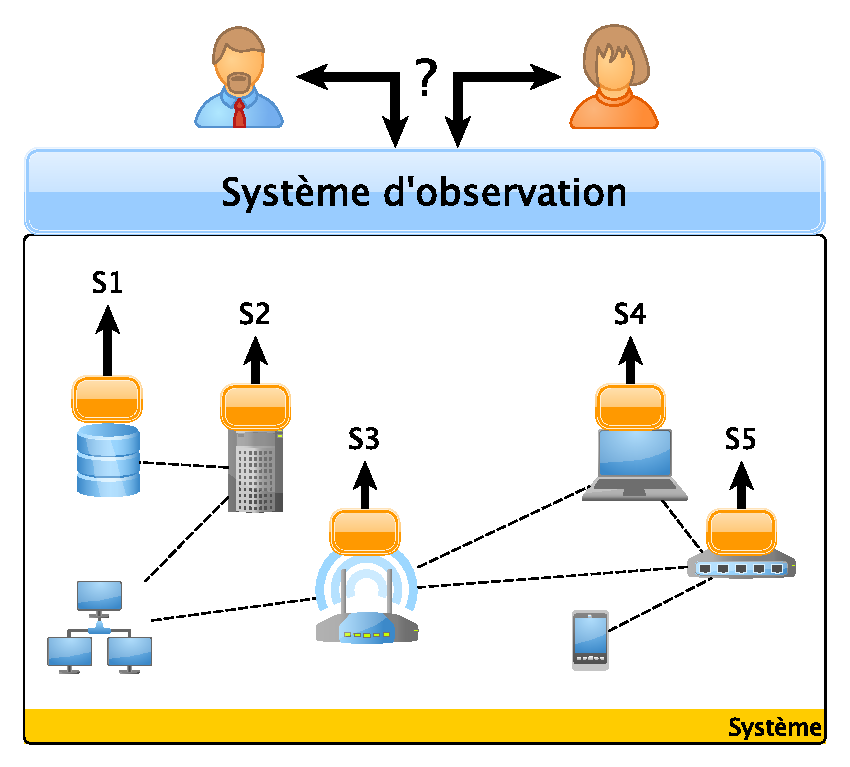
\includegraphics[width=0.5\textwidth]{intro-objectif2}
\caption{Représentation d'un système observé par deux utilisateurs}\label{fig:intro:objectif:abstraction}
\end{figure}

\subsection{Hétérogénéité des données des systèmes observés}\label{sec:intro:problematique:data}
Dans notre contexte, nous identifions deux types d'hétérogénéités : l'hétérogénéité structurelle des données, et l'hétérogénéité en terme de dynamisme.
\subsubsection{Descriptions hétérogènes des systèmes}
Tout système peut être décrit par un \textbf{schéma conceptuel} fixant une sémantique. Ce schéma s'appuie sur un \textbf{modèle de données} théorique tels que : le modèle hiérarchique, le modèle réseaux sémantiques, le modèle relationnel ou encore le modèle objet. Ainsi, chaque système observé s'abstrait par un schéma différent et l'observation doit pouvoir s'adapter à chacun d'eux.

De plus, le système expose un ensemble de sources de données hétérogènes, car chacune possède son propre schéma. Il est nécessaire d'\textbf{intégrer} ces données pour que celles-ci puissent être manipulés par le schéma du système.

\subsubsection{Évolution des données}
Le système observé évolue au fur et à mesure du temps. Ce dynamisme introduit le problème de la gestion de deux catégories différentes de données. En effet, il existe deux grandes \textbf{catégories de données} : les données \textbf{persistantes} et les données \textbf{temps réel}. Les données persistantes sont à évolution lente et les données temps réel sont des relevés instantanés et très volatiles indiquant l'état du système (sous forme de flux de données).

Néanmoins, chacune de ces catégories possède des modèles de données et des traitements propres. Or, ces données proviennent toutes du même système, qu'elles soient temps réel ou persistantes. Il existe des liens entre ces deux catégories de données. L'expérience montre que l'archivage d'un flux permet d'extraire de nouvelles connaissances par analyse de son historique. À l'inverse, une donnée stockée peut subir des modifications déclenchant la production d'événements, ce qui est assimilable à un flux de données.

Ces processus de traitements de données sont assimilables à des requêtes d'interrogation que pose l'utilisateur sur l'ensemble des données. Il existe différent \textbf{modes d'interrogations} (ou requêtes) qui, d'une certaine manière, reflètent l'hétérogénéité de l'évolution des données.
\begin{itemize}
    \item \textbf{Interrogation instantanée} : C'est la manière usuelle d'interroger dans les applications de gestion de base de données. L'utilisateur pose une question sur un ensemble de données considérées figées, du moins le temps du calcul de la réponse. Le système fournit une réponse représentative d'un état à un instant donné. Par exemple : \enquote{\it quel est l'ensemble actuel des équipements actifs de mon système}. La réponse à cette requête pourrait être \enquote{\it à cet instant, les équipements Box, PC1 et STB sont connectés et actifs}. La mention \enquote{\it à cet instant} est très importante, car si un nouvel équipement arrive dans le système, une nouvelle évaluation donnerait une réponse différente. Ainsi, cette interrogation correspond à la consultation ponctuelle de l'ensemble des données disponibles.
    \item \textbf{Interrogation continue} : Les données sont considérées en constante évolution. L'utilisateur obtient ainsi une réponse qui évolue au cours du temps, sous forme de flux ou de mise à jour d'état. La durée de vie de ce processus peut être indéfini. Un exemple pouvant être : \enquote{\it toutes les minutes, le flux de la charge moyenne sur une minute du processeur du PC1}. La réponse forme un flux continu d'information qui, toutes les minutes, reporte une nouvelle valeur moyenne pour ce capteur. La formation de processus de collecte ou de formation d'alerte suit ce type d'interrogation.
\end{itemize}

Il est important de noter que ces deux méthodes d'interrogation peuvent se combiner pour exécuter une requête hybride. Par exemple, il est possible d'effectuer un appel à une interrogation instantanée à l'intérieur d'un processus continu. De façon similaire, l'appel régulier d'une interrogation instantanée forme une réponse continue. Il est nécessaire que le système d'observation soit capable de manipuler naturellement ces deux types d'interrogation pour refléter correctement le dynamisme du système observé.

\subsection{Caractéristiques du système d'observation}\label{sec:intro:problematique:monitoring}
La capacité à s'adapter à l'application finale est un point important de la mise en œuvre d'un système d'observation. Plus la portée de l'observation est générique plus ce critère est critique. Ainsi, il est important que le nombre et la complexité des procédures nécessaires à l'adaptation au système visé soient faibles. Car, si un système est complet, mais nécessite une adaptation longue et complexe, il devient difficile à mettre en pratique.

\subsubsection{Langage de manipulation de données}
Afin de pouvoir intégrer et interroger les données, le système d'observation doit se doter de capacités de traitements des données. L'\textbf{expression} des traitements possibles se fait à travers un \textbf{langage}. Pour plus de flexibilité, nous souhaitons nous extraire le plus possible des algorithmes de traitement de données, ainsi les \textbf{paradigmes} déclaratifs sont privilégiés. Le langage utilisé peut avoir un \textbf{pouvoir d'expression} limité. Il est important d'être capable d'énumérer ce qui est possible d'exprimer. Les classes de logiques ou les équivalences à d'autres langages permettent de caractériser ces limitations.

Pour que le système d'observation perturbe le moins possible le système observé, il est nécessaire que l'évaluation de ce langage soit \textbf{performant}. De plus, ce critère améliore la qualité des réponses en terme de latence de traitement. Le critère se mesure sur la capacité à traiter la charge d'un système en terme de nombre de sources ou en terme de débit supporté.

\subsubsection{Adaptabilité aux besoins}
Afin de pouvoir s'adapter aux besoins des utilisateurs, il est nécessaire que le système d'observation soit capable d'utiliser des \textbf{routines spécifiques} de traitement de données fournies par l'utilisateur. Cette extensibilité permet aussi bien l'intégration de tous types de besoins que l'amélioration des performances de traitements récurrents.

Enfin, il existe plusieurs \textbf{perspectives} possibles à un système. En fonction de son expérience, de ses connaissances ou de ses intérêts, chaque utilisateur perçoit le système à sa manière. Cet angle de vue définit les données surveillées, en établissant des préférences sur ce qui est observé. Mais cela peut influencer aussi la représentation du système observé. Il est nécessaire que le système d'observation s'adapte aux perspectives dans lesquelles se placent les utilisateurs.

En conclusion, la problématique de cette thèse est d'observer un système générique en étant capable de s'adapter à sa dynamique, à son hétérogénéité, tout en restant ouvert aux traitements spécifiques d'une application.
